% sage_latex_guidelines.tex V1.20, 14 January 2017

\documentclass[Review,sagev,times]{sagej}
%\documentclass[Afour,sagev,times]{sagej}

\usepackage{moreverb,url}

\usepackage[colorlinks,bookmarksopen,bookmarksnumbered,citecolor=red,urlcolor=red]{hyperref}
\usepackage{caption}
\usepackage{pdfpages}
\usepackage[tbtags]{amsmath}

\PassOptionsToPackage{tbtags}{amsmath}

\newcommand\BibTeX{{\rmfamily B\kern-.05em \textsc{i\kern-.025em b}\kern-.08em
T\kern-.1667em\lower.7ex\hbox{E}\kern-.125emX}}

\DeclareMathOperator{\argmax}{arg\,max}

\def\volumeyear{2018}

\begin{document}

\runninghead{Tomer et al.}

\title{Personalized Decision Making for Biopsies in Prostate Cancer Active Surveillance Programs}

\author{Anirudh Tomer\affilnum{1}, Daan~Nieboer\affilnum{2}, Monique~J.~Roobol\affilnum{3}, Ewout~W.~Steyerberg\affilnum{2,4}, and Dimitris~Rizopoulos\affilnum{1}}

\affiliation{\affilnum{1}Department of Biostatistics, Erasmus University Medical Center, the Netherlands\\
\affilnum{2}Department of Public Health, Erasmus University Medical Center, the Netherlands\\
\affilnum{3}Department of Urology, Erasmus University Medical Center, the Netherlands\\
\affilnum{4}Department of Medical Statistics and Bioinformatics, Leiden University Medical Center, The Netherlands}

\corrauth{Anirudh Tomer, 
Erasmus MC,
t.a.v. Anirudh Tomer / kamer Na-2701,
PO Box 2040,
3000 CA Rotterdam,
the Netherlands.}

\email{a.tomer@erasmusmc.nl}

% !TEX root =  ../main_manuscript.tex 
\begin{abstract}
\texttt{Objective}: To develop a model and methodology for predicting the risk of Gleason \emph{upgrading} in prostate cancer active surveillance (AS) patients, and using the predicted risks to create risk-based \emph{personalized} biopsy schedules as an alternative to one-size-fits-all schedules (e.g., annually). Furthermore, to assist patients and doctors in making shared decisions of biopsy schedules, by providing them quantitative estimates of the \emph{burden} and \emph{benefit} of opting for personalized versus any other schedule in AS. Last, to externally validate our model and implement it along with personalized schedules in a ready to use web-application.\\

\texttt{Materials and Methods}: We used longitudinal prostate-specific antigen (PSA) measurements, timing and results of previous biopsies, and age at baseline from the world's largest AS study, Prostate Cancer Research International Active Surveillance or PRIAS (7813 patients, 1134 experienced upgrading). We fitted a Bayesian joint model for time-to-event and longitudinal data to the PRIAS dataset. We then externally validated our model in the largest six AS cohorts of the Movember Foundation's Global Action Plan (GAP3) database (${>20,000}$ patients, 27 centers worldwide), covering nearly 73\% of all GAP3 patients. We used the predicted upgrading-risks from the validated models to schedule biopsies whenever a patient's risk of upgrading was above a certain threshold. To assist patients in choice of this threshold to compare the resulting schedule with currently practiced schedules, we provided them the timing and the total number of biopsies (burden) planned, and the predicted time delay in detecting upgrading (shorter is better) for each schedule.\\

\texttt{Results}: The cause-specific cumulative upgrading-risk at year five of follow-up was 35\% in PRIAS, and at most 50\% in GAP3 cohorts. In the PRIAS based model, PSA velocity was a stronger predictor of upgrading (Hazard~Ratio:~2.47, 95\%CI:~1.93--2.99) than PSA value (Hazard~Ratio:~0.99, 95\%CI:~0.89--1.11). Our model had a moderate area under the receiver operating characteristic curve (0.6--0.7) in validation cohorts. The prediction error was moderate (0.1--0.2) in GAP3 cohorts where the impact of PSA value and velocity on upgrading-risk was similar to PRIAS, but large (0.2--0.3) otherwise. Our model required recalibration of baseline upgrading-risk in validation cohorts. We used predicted upgrading-risk from the validated model to create personalized biopsy schedules for real AS patients and implemented them in a web-application (\url{http://tiny.cc/biopsy}).\\

\texttt{Conclusions}: We successfully developed and validated a model for predicting upgrading-risk, and providing risk-based personalized biopsy decisions, in prostate cancer AS. Personalized prostate biopsies are a novel alternative to fixed one-size-fits-all schedules that may help to reduce unnecessary prostate biopsies while maintaining cancer control. The model and schedules made available via a web-application enable shared decision making of biopsy schedules by comparing fixed and personalized schedules on total biopsies and expected time delay in detecting upgrading.
\end{abstract}

\keywords{Active surveillance, biopsy, joint models, personalized medicine, prostate cancer}

\maketitle

\footnote{Financial support for this study was provided Netherlands Organization for Scientific Research's VIDI grant nr. 016.146.301, and Erasmus MC funding. The funding agreement ensured the authors’ independence in designing the study, interpreting the data, writing, and publishing the report.\\Word Count: 4046}
\thefootnote

% !TEX root =  ../main_manuscript.tex 
\section{Introduction}
\label{sec:introduction}
Chronic non-communicable diseases (e.g., cancer, renal, cardiovascular diseases, etc.) are the primary cause of human deaths worldwide~\citep{alwan2010monitoring}. After diagnosis, in many such patients, surveillance tests are performed periodically to detect disease \textit{progression}, a non-terminal event. Often the most accurate or gold standard surveillance tests are also invasive. For example, to diagnose progression, biopsies are conducted repeatedly in prostate cancer~\citep{bokhorst2015compliance}, endoscopies in Barrett's esophagus~\citep{streitz1993endoscopic}, and colonoscopies in colorectal cancer~\citep{krist2007timing}. Repeat biopsies are also utilized to detect allograft deterioration in lung~\citep{mcwilliams2008surveillance} and kidney transplant~\citep{henderson2011surveillance} patients.

Usually, invasive tests are scheduled in a fixed manner, e.g., every six months. Test frequency varies between diseases~\citep{henderson2011surveillance,bokhorst2015compliance,krist2007timing} and cohorts. Although, due to the periodical nature of test schedules, progression is always detected with a time delay (Figure~\ref{fig:delay_explanation}). This time delay can be reduced by scheduling tests frequently. However, invasive tests are difficult to conduct, can lead to severe complications~\citep{loeb2013systematic,krist2007timing}, cause patient discomfort, and sometimes patients may not comply with frequent tests~\citep{bokhorst2015compliance}. In this regard, fixed test schedules ignore the differences in speed of progression between patients, and impose an equal medical burden on all. Hence, the frequency of invasive tests holds important implications for patients.

\begin{figure}
\centerline{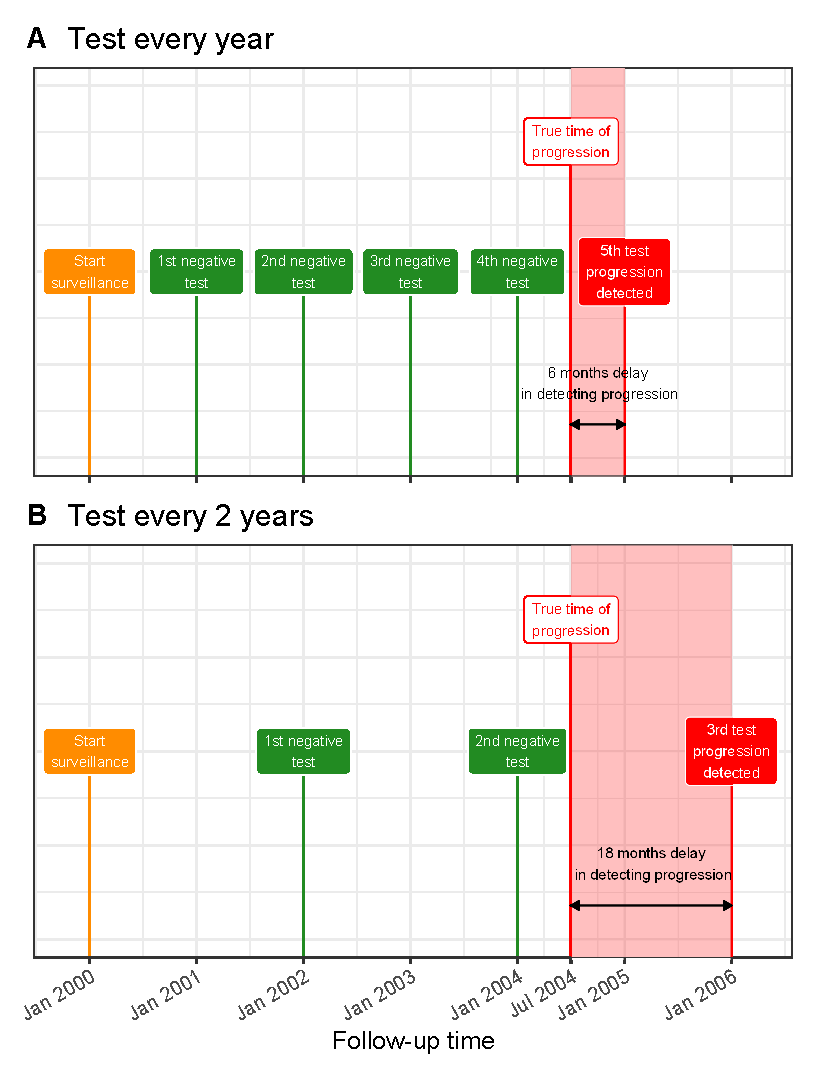
\includegraphics{images/delay_explanation.eps}}
\caption{\textbf{Trade-off between the number of invasive tests and time delay in detecting progression (non-terminal event of interest):} The true time of progression for this patient July 2004. More frequent invasive tests in \textbf{Panel~A} lead to a smaller time delay in detection of progression than less frequent invasive tests in \textbf{Panel~B}. Since invasive tests are conducted periodically, the time of progression is observed as an interval. For example, between Jan~2004--Jan~2005 in \textbf{Panel~A} and between Jan~2004--Jan~2006 in \textbf{Panel~B}.} 
\label{fig:delay_explanation}
\end{figure}

In this paper, we aim to balance the number of invasive tests (burden) and the time delay in detection of \textit{progression} (less is beneficial) better than fixed schedules. For this purpose, we intend to create personalized test schedules that exploit patient-specific clinical data accumulated during follow-up. This data includes baseline characteristics of patients; results from previous invasive tests; and longitudinal biomarker, physical examination, and medical imaging measurements, etc. Previous approaches for personalized schedules may be divided into three categories. First, heuristic methods such as decision making flowcharts, e.g.,~\citet{bokhorst2015compliance}. However, flowcharts discretize continuous clinical outcomes, often utilize only the latest data point, and ignore the measurement error in observed outcomes. Second, personalized test decisions employing partially observable Markov decision processes~\citep{alagoz2010operations, steimle2017markov}. Although, their application with continuous outcomes is limited by the curse of dimensionality. Third, personalized schedules obtained by optimizing a loss function of clinical parameters of interest~\citep{bebu2017optimal,rizopoulos2015personalized}, including our previous work on scheduling biopsies in prostate cancer~\citep{tomer2019personalized}. In this work, we will employ the third approach.

First, we develop a full specification of the joint distribution of patient-specific longitudinal clinical outcomes and time of \textit{progression}. We achieve this using joint models for time-to-event and longitudinal data~\citep{tsiatis2004joint,rizopoulos2012joint}. We use joint models because they are inherently personalized. Specifically, they exploit patient-specific random effects~\citep{laird1982random} to model longitudinal outcomes without discretizing them. We subsequently employ the fitted joint model for new patients, to estimate their patient-specific cumulative-risk over their current and future follow-up visits. These risk predictions utilize their clinical data accumulated until their latest follow-up. We then schedule invasive tests on all those future follow-up visits where a patient's conditional cumulative-risk of progression is above a certain threshold (e.g., 10\% risk). We also automate the choice of this threshold and the resulting schedule. More specifically, we optimize a function of the number of tests in a schedule and the expected time delay in the detection of progression. We estimate this delay in a patient-specific manner for both fixed and personalized schedules, thus facilitating shared-decision making of invasive test schedules.

This research is motivated by the problem of scheduling biopsies~\citep{nieboer2018active} in the world's largest prostate cancer active surveillance study PRIAS~\citep{bokhorst2015compliance}. It has 7813 patients, 104904 longitudinal measurements, and 1134 patients with cancer progression. Patients in PRIAS have low and very-low grade prostate cancer, often over-diagnosed due to prostate-specific antigen (PSA) based screening tests~\citep{crawford2003epidemiology}. The goal of surveillance is to delay serious treatments (e.g., surgery, chemotherapy, etc.) until cancer progression is observed. For this purpose, patients are monitored continually via PSA (ng/mL) blood tests, digital rectal examination (DRE) for shape and size of the tumor, and biopsy Gleason grade group~\citep{epsteinGG2014}. The latter is the strongest indicator of cancer-related outcomes. Consequently, treatment is commonly advised upon observing an increase in a patient's biopsy Gleason grade group (cancer progression). Currently, the most common biopsy schedule of yearly biopsies~\citep{loeb2014heterogeneity} leads to many unnecessary biopsies in slow/non-progressing patients (50\% proportion in some cohorts). Biopsy burden combined with patient non-compliance to frequent biopsies~\citep{bokhorst2015compliance} has raised concerns regarding the optimal biopsy schedule. Since prostate cancer has the second highest incidence among all cancers in males~\citep{GlobalCancerStats2012}, biopsy schedules tailored for individual patients can reduce the overall burden of biopsies in a large number of patients worldwide.

The rest of the paper is as follows. Section~\ref{sec:jointmodel} briefly introduces the joint modeling framework. In Section~\ref{sec:schedule} we present the methodology for personalized schedules, and then demonstrate them for biopsies in real PRIAS patients in Section~\ref{sec:results}. Lastly, in Section~\ref{sec:sim_study} we show the efficacy of personalized schedules via a realistic simulation study based on PRIAS patients.
% !TEX root =  ../main_manuscript.tex

\section{Methods}
\label{sec:methods}
\subsection{Study Population}
To develop our methodology we use data of the patients of the PRIAS study (\url{www.prias-project.org}). The dataset consists of 5270 patients, of which 866 observe cancer progression. For each patient, PSA measurements (ng/mL) are scheduled every 3 months for the first 2 years and every 6 months thereafter. The DRE measurements are scheduled every 6 months. We use the DRE measurements after converting them on a binary scale, namely $\mbox{DRE} > \mbox{T1c}$ and $\mbox{DRE} \leq \mbox{T1c}$ \cite{schroder1992tnm}. On average 5 DRE and 9 PSA measurements have been recorded per patient. In order to identify cancer progression, biopsies are scheduled as per the PRIAS protocol (see \hyperref[sec:introduction]{Introduction}).

\subsection{A Bivariate Joint Model for the Longitudinal PSA, and DRE Measurements, and Time to Cancer Progression}
Let $T_i^*$ denote the true cancer progression time for the $i$-th patient in PRIAS. Since biopsies are conducted periodically, $T_i^*$ cannot be observed directly and it is only known to fall in an interval ${l_i < T_i^* \leq r_i}$, where $r_i$ and $l_i$ are the time of the latest and second latest biopsies, respectively, if the progression is observed at the latest biopsy. When the progression is not observed, then $l_i$ is the time of the latest biopsy and $r_i = \infty$. Further, let $\boldsymbol{y}_{di}$, and $\boldsymbol{y}_{pi}$ denote the $n_{di} \times 1$, and $n_{pi} \times 1$ vectors of the DRE, and PSA longitudinal measurements, respectively. For a sample of $n$ patients the observed data is denoted by ${\mathcal{D}_n = \{l_i, r_i, \boldsymbol{y}_{di}, \boldsymbol{y}_{pi}; i = 1, \ldots, n\}}$.

The patient-specific PSA and DRE measurements over time are modeled using a generalized linear mixed effects model. For the $i$-th patient, the mixed effects sub-model for DRE is given by:
\begin{equation}
\label{eq:long_model_dre}
\begin{split}
    \mbox{logit} \big[\mbox{Pr}\{y_{di}(t) > \mbox{T1c}\}\big] &= \beta_{0d} + b_{0di} + (\beta_{1d} + b_{1di}) t\\
    &+ \beta_{2d} (\mbox{Age}_i-70) + \beta_{3d} (\mbox{Age}_i-70)^2
    \end{split}
\end{equation}
where, $t$ denotes a specific time point in the AS follow-up, $\mbox{Age}_i$ is the age of the $i$-th patient at the time of inclusion in AS. The fixed effect parameters are denoted by $\{\beta_{0d}, \ldots, \beta_{3d}\}$, and $b_{0di}, b_{1di}$ are the patient specific random effects. With this definition, we assume that the log odds of obtaining a DRE score larger than T1c remain linear over time. An example model fit for DRE is shown in panel A of Figure~\ref{fig:jmExplanationPlot_1757}. For the $i$-th patient, the mixed effects sub-model for PSA is given by:
\begin{equation}
\label{eq:long_model_psa}
\begin{split}
    \log_2 \big\{y_{pi}(t) + 1\big\} &= m_{pi}(t) + \varepsilon_{pi}(t),\\
    m_{pi}(t) &= \beta_{0p} + b_{0pi} + \sum_{k=1}^4 (\beta_{kp} + b_{kpi})  B_k(t,\mathcal{K})\\ 
    &+ \beta_{5p} (\mbox{Age}_i-70) + \beta_{6p} (\mbox{Age}_i-70)^2,
    \end{split}
\end{equation}
where, $m_{pi}(t)$ denotes the underlying measurement error free value of $\log_2 (\mbox{PSA} + 1)$ transformed \citep{pearson1994mixed,lin2000latent} measurements at time $t$. To accommodate for a non-linear evolution of this value over the follow-up period in AS, we utilize B-splines \citep{de1978practical}. In Equation (\ref{eq:long_model_psa}), $B_k(t, \mathcal{K})$ denotes the $k$-th basis function of a B-spline with three internal knots at $\mathcal{K} = \{0.1, 0.7, 4\}$ years, and boundary knots at 0 and 5.42 years (0.95 quantile of the observed follow-up times). The fixed effect parameters are denoted by $\{\beta_{0p},\ldots,\beta_{6p}\}$ and the patient specific random effects are denoted by $\{b_{0pi}, \ldots, b_{4pi}\}$. The error $\varepsilon_{pi}(t)$ is assumed to be t-distributed with three degrees of freedom (see Appendix~B.1) and scale $\sigma$, and is independent of the random effects. An example model fit for PSA is shown in panel B of Figure~\ref{fig:jmExplanationPlot_1757}. To account for the association between the DRE and PSA measurements, we link their corresponding random effects. More specifically, the complete vector of random effects ${\boldsymbol{b}_i = (b_{0di}, b_{0di}, b_{0pi}, \ldots, b_{4pi})^T}$ is assumed to follow a multivariate normal distribution with mean zero and ${7\times 7}$ variance-covariance matrix $\boldsymbol{D}$.
\begin{figure}[!htb]
\captionsetup{justification=justified}
\centerline{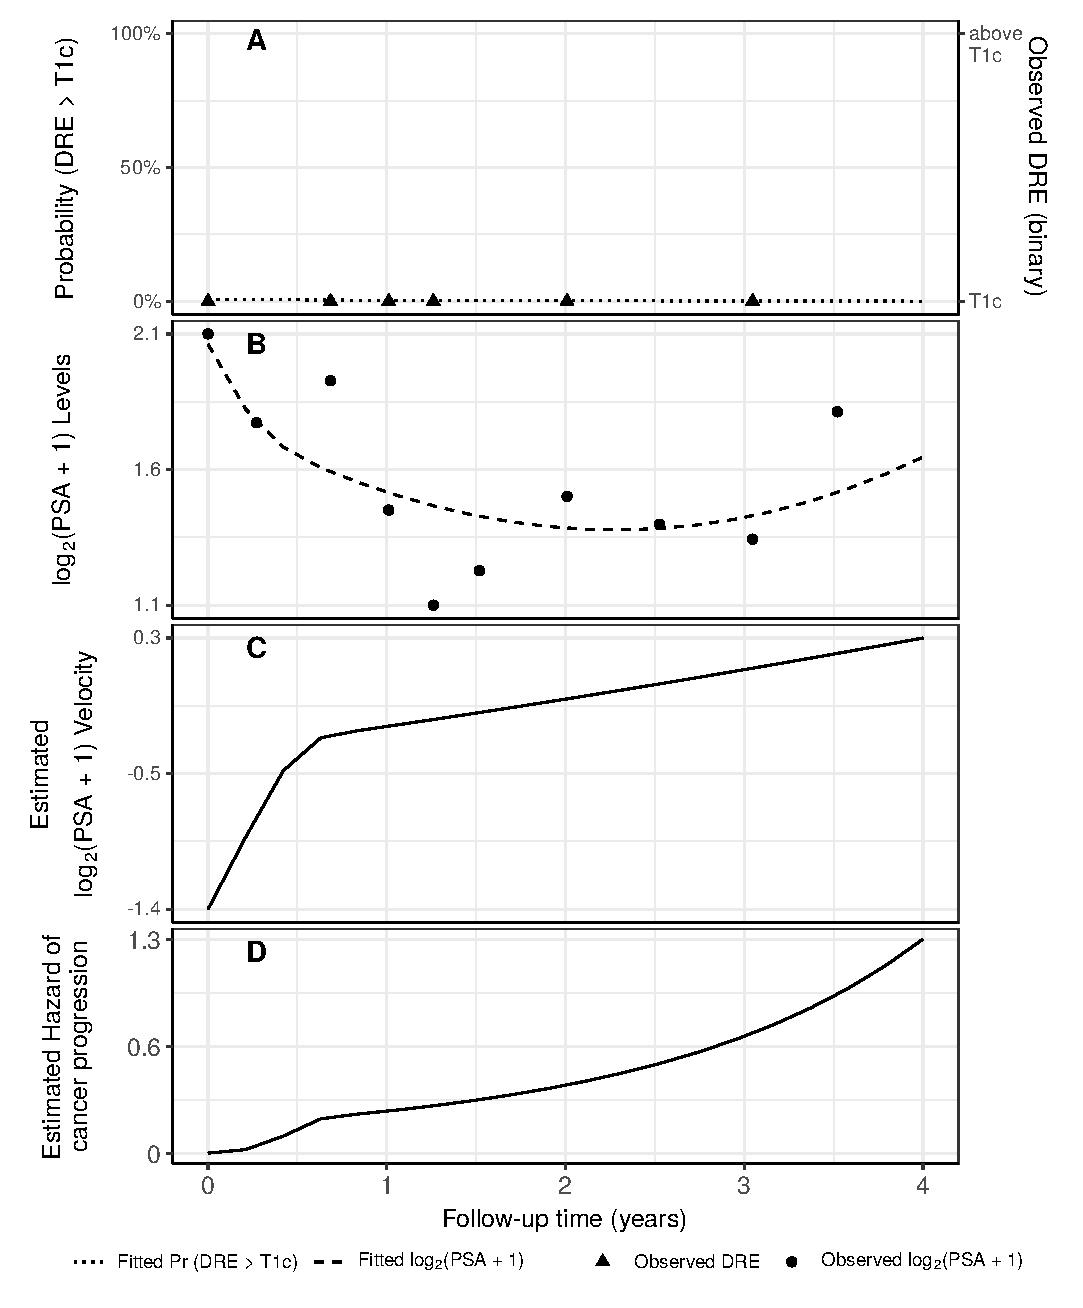
\includegraphics[width=\columnwidth]{images/jmExplanationPlot_1757.eps}}
\caption{Illustration of the joint model fitted to the PRIAS dataset. \textbf{Panel~A:} shows the observed DRE scores and the fitted probability of obtaining a DRE score greater than T1c (Equation~\ref{eq:long_model_dre}). \textbf{Panel~B:} shows the observed and fitted $\log_2(\mbox{PSA} + 1)$ levels (Equation~\ref{eq:long_model_psa}). \textbf{Panel~C:} shows the estimated $\log_2(\mbox{PSA} + 1)$ velocity (velocity cannot be observed directly) over time. The hazard function (Equation~\ref{eq:rel_risk_model}) shown in \textbf{Panel~D}, depends on the fitted log odds of having a $\mbox{DRE} > \mbox{T1c}$, and the fitted $\log_2(\mbox{PSA} + 1)$ value and velocity.}
\label{fig:jmExplanationPlot_1757}
\end{figure}

To model the impact of DRE and PSA measurements on the risk of cancer progression, we use a relative risk sub-model. More specifically, the hazard of cancer progression $h_i(t)$ at a time $t$ is given by:
\begin{equation}
\label{eq:rel_risk_model}
\begin{split}
    h_i(t) &= h_0(t) \exp\Big(\gamma_1 (\mbox{Age}_i-70) + \gamma_2 (\mbox{Age}_i-70)^2\\
    &+\alpha_{1d} \times \mbox{logit} \big[\mbox{Pr}\{y_{di}(t) > \mbox{T1c}\}\big]+ \alpha_{1p} \times m_{pi}(t) + \alpha_{2p} \times \frac{\partial m_{pi}(t)}{\partial {t}}\Big),
    \end{split}
\end{equation}
where, $\gamma_1, \gamma_2$ are the coefficients for the effect of age. The parameter $\alpha_{1d}$ models the impact of log odds of obtaining $\mbox{DRE} > \mbox{T1c}$ on the hazard of cancer progression. The impact of PSA on the hazard of cancer progression is modeled in two ways, namely at any time $t$ the effect of the instantaneous underlying value (dashed line in panel B of Figure~\ref{fig:jmExplanationPlot_1757}) of PSA $m_{pi}(t)$ is given by $\alpha_{1p}$, and the effect of the instantaneous underlying PSA velocity $\partial m_{pi}(t)/\partial {t}$ (panel C in Figure~\ref{fig:jmExplanationPlot_1757}) is given by $\alpha_{2p}$. Lastly, $h_0(t)$ is the baseline hazard at time $t$, and is modeled flexibly using P-splines \citep{eilers1996flexible}. An example fitted hazard is shown in Panel D of Figure~\ref{fig:jmExplanationPlot_1757}. The detailed specification of the baseline hazard $h_0(t)$, and parameter estimation using the Bayesian approach are presented in Appendix A of the supplementary material.

\subsection{Personalized Decisions for Biopsy During Follow-up Visit}
\label{subsec:pers_decision_making}
Let us assume that a decision of conducting a biopsy is to be made for a new patient $j$, who is not present in the PRIAS dataset. Let $t$ be the time of his latest biopsy, and $s$ denotes the current follow-up visit time. Let $\mathcal{Y}_{dj}(s)$ and $\mathcal{Y}_{pj}(s)$ denote the vector of all DRE and PSA measurements taken up to the current visit $s$, respectively. From the observed measurements we want to extract the underlying measurement error free trend of $\log_2 (\mbox{PSA} + 1)$ values and velocity, and the log odds of obtaining $\mbox{DRE} > \mbox{T1c}$. We intend to combine them to inform us when the cancer progression is to be expected (see Figure~\ref{fig:dynRiskPlot_2340}), and to further guide the decision making on whether to conduct a biopsy at the current follow-up visit. The combined information is given by the posterior predictive distribution $g(T^*_j)$ of the time of cancer progression $T^*_j$. It is given by:
\begin{equation*}
\label{eq:post_pred_dist}
\begin{aligned}
g(T^*_j) &= p\big\{T^*_j \mid T^*_j > t, \mathcal{Y}_{dj}(s), \mathcal{Y}_{pj}(s), \mathcal{D}_n\big\}\\
&= \int \int p\big(T^*_j \mid T^*_j > t, \boldsymbol{b}_j, \boldsymbol{\theta}\big)\\
&\times p\big\{\boldsymbol{b}_j \mid T^*_j>t, \mathcal{Y}_{dj}(s), \mathcal{Y}_{pj}(s), \boldsymbol{\theta}\big\}p\big(\boldsymbol{\theta} \mid \mathcal{D}_n\big) \mathrm{d} \boldsymbol{b}_j \mathrm{d} \boldsymbol{\theta}.
\end{aligned}
\end{equation*}
The distribution $g(T^*_j)$ updates as extra information is recorded at follow-up visits. It is also unique for each patient as it depends on the historical data of the patient via the posterior distribution of the random effects $\boldsymbol{b}_j$.

A key ingredient in the decision of conducting a biopsy at the current follow-up visit time $s$, is the risk that the cancer has already progressed since the time of the last biopsy $t$ (see Figure~\ref{fig:dynRiskPlot_2340} for illustration). This risk can be derived from the posterior predictive distribution $g(T^*_j)$ \cite{rizopoulos2011dynamic}, and is given by:
\begin{equation*}
\label{eq:dynamic_risk_prob}
R_j(s \mid t) = \mbox{Pr}\big\{T^*_j \leq s \mid T^*_j > t, \mathcal{Y}_{dj}(s), \mathcal{Y}_{pj}(s), \mathcal{D}_n\big\}, \quad s \geq t.
\end{equation*}
\begin{figure}[!htb]
\captionsetup{justification=justified}
\centerline{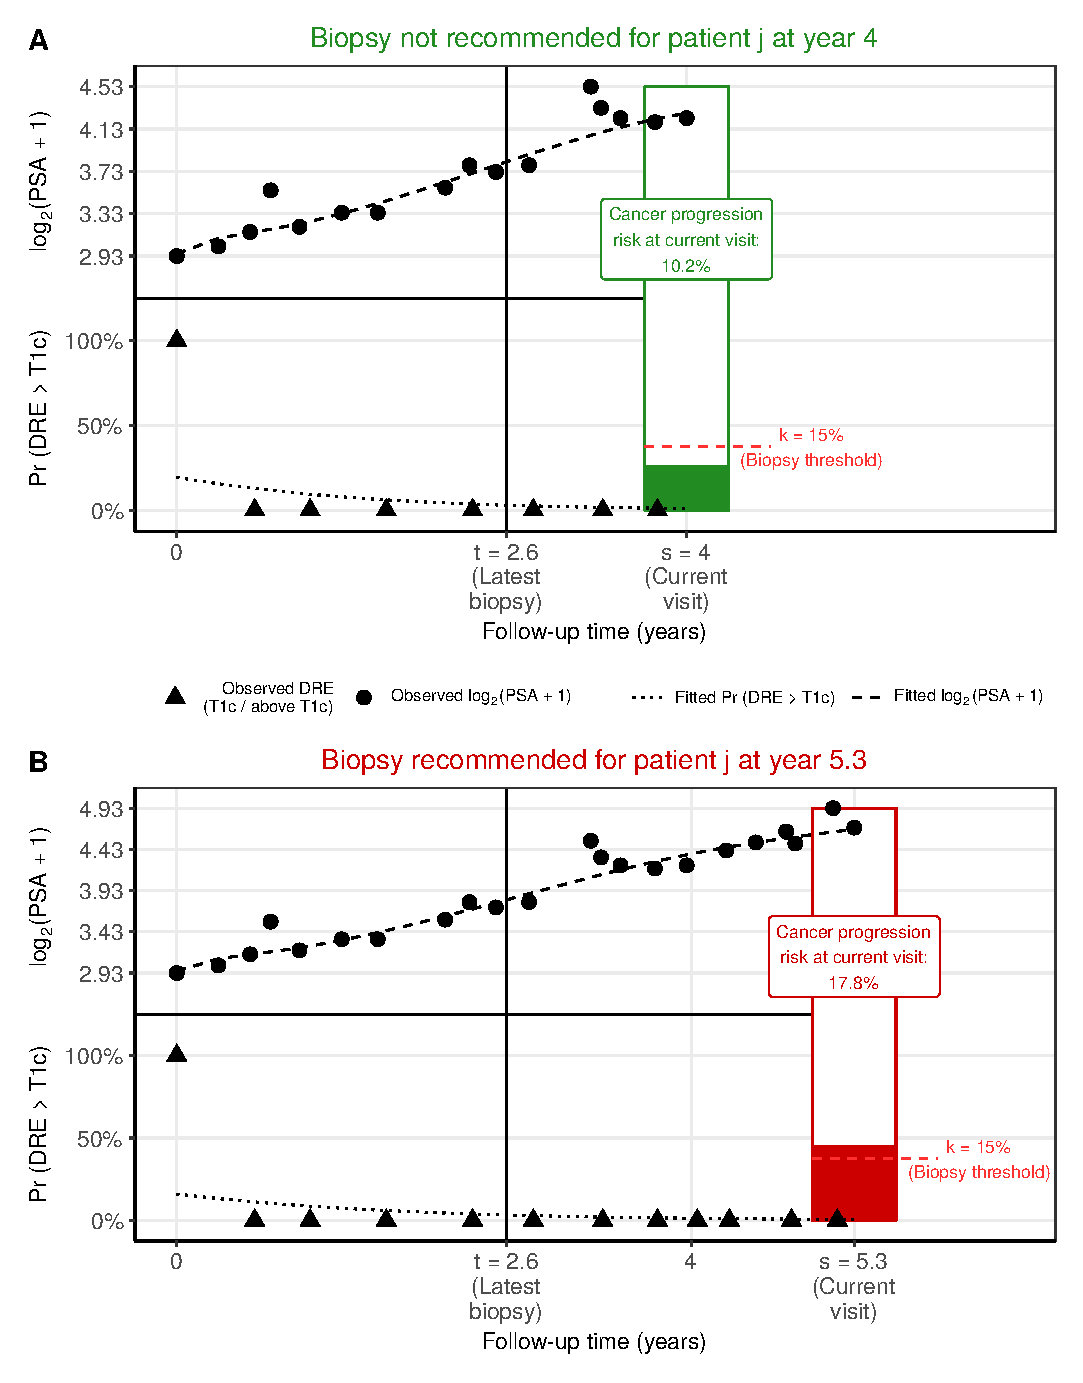
\includegraphics[width=\columnwidth]{images/dynRiskPlot_2340.eps}}
\caption{Illustration of personalized decision making for patient $j$ at two different follow-up visits. Biopsy is recommended if the risk of cancer progression estimated from the joint model fitted to the PSA and DRE measurements of the patient, is higher than the example risk threshold for biopsy ($\kappa=$ 15\%). \textbf{Panel~A:} biopsy is not recommended for the patient $j$ at the follow-up visit time $s=4$ years, because his estimated risk of cancer progression (10.2\%) is less than the biopsy risk threshold. \textbf{Panel~B:} biopsy is recommended for the patient $j$ at the follow-up visit time $s=5.3$ years, because his estimated risk of cancer progression (17.8\%) is more than the biopsy risk threshold.}
\label{fig:dynRiskPlot_2340}
\end{figure}
A simple and straightforward approach to decide upon conducting a biopsy at a follow-up visit would be to do so when the risk of cancer progression at that visit is higher than a certain threshold $0 \leq \kappa \leq 1$. For example, as shown in panel B of Figure~\ref{fig:dynRiskPlot_2340}, biopsy at a follow-up visit may be scheduled if the risk is higher than 15\% (example risk threshold). Since there are infinite possible risk thresholds between 0\% and 100\% risk, the choice of a single threshold at a follow-up visit can become dilemmatic for patients/doctors.

In such situations, we propose an alternative approach of automatic selection of thresholds. Using information from the observed cancer progression times in the PRIAS dataset, at a follow-up visit a threshold is chosen on the basis of its ability to discriminate between patients who obtain cancer progression versus others. More specifically, given the time $t$ of the latest biopsy we propose to choose a threshold $\kappa$ for which a binary classification accuracy measure \citep{lopez2014optimalcutpoints}, discriminating between patients observing cancer progression (positive result) versus others (negative result), is maximized. In joint models, a patient $j$ is predicted to have progression in the time period $(t, s]$ between the current visit and the last biopsy, if ${R_j(s \mid t) > \kappa}$ \cite{rizopoulosJMbayes, landmarking2017}. Otherwise the patient is predicted to not have progression. Since we are interested in detecting cancer progressions, we can choose a $\kappa$ for which the true positive rate (also known as sensitivity, or probability of detection) is maximized. However, this may lead to a high false positive rate as well (unnecessary biopsy suggestions). This issue can be mitigated by maximizing for the positive predictive value (also known as precision) simultaneously. To this end, we utilize the $\mbox{F}_1$ score, which is a composite of time dependent true positive rate (TPR) and positive predictive value (PPV), and is defined as:
\begin{equation}
\label{eq:F1_TPR_PPV}
\begin{split}
\mbox{F}_1(t,  s, \kappa) &= 2\frac{\mbox{TPR}(t,  s, \kappa)\ \mbox{PPV}(t,  s, \kappa)}{\mbox{TPR}(t,  s, \kappa) + \mbox{PPV}(t,  s, \kappa)},\\
\mbox{TPR}(t,  s, \kappa) &= \mbox{Pr}\big\{R_j(s \mid t) > \kappa \mid t < T^*_j \leq s\big\},\\
\mbox{PPV}(t,  s, \kappa) &= \mbox{Pr}\big\{t < T^*_j \leq s \mid R_j(s \mid t) > \kappa \big\}.
\end{split}
\end{equation}
The $\mbox{F}_1$ score ranges between 0 and 1, where a value of 1 signifies perfect TPR and PPV. Since a high $\mbox{F}_1$ score is desired, the value of biopsy threshold $\kappa$ is $\argmax_{\kappa} \mbox{F}_1(t, s, \kappa)$. The time dependent TPR and PPV are estimated from the joint model fitted to the PRIAS dataset \cite{landmarking2017}.

\subsection{Simulation Study}
Although the personalized decision making approach is motivated by the PRIAS study, it is not possible to evaluate it on the PRIAS dataset. This is due to the fact that the PRIAS patients have already had their biopsies as per the PRIAS protocol. In addition, the true time of cancer progression is interval or right censored for all patients, making it impossible to correctly estimate the delay in detection of cancer progression due to a particular schedule. To this end, we conduct an extensive simulation study to compare personalized, PRIAS and annual schedules. For a realistic comparison, we simulate data from the joint model fitted to the PRIAS dataset. The simulated population has the same follow-up period of 10 years as the PRIAS study. In addition the recovered relations between PSA and DRE measurements, and the risk of cancer progression, are retained in the simulated population.

From this population, we first sample 500 datasets with 1000 patients each. We generate a true cancer progression time for each of the patients, and then sample a set of PSA and DRE measurements at the same time points as given in PRIAS protocol. We then split each dataset into a training (750 patients) and a test (250 patients) part, and generate a random and non‐informative censoring time for the training patients. We next fit a joint model of the specification given in Equation (\ref{eq:long_model_dre}), (\ref{eq:long_model_psa}) and (\ref{eq:rel_risk_model}) to each of the 500 training datasets and obtain MCMC samples from the 500 sets of the posterior distribution of the parameters. Using these fitted joint models, we obtain the posterior predictive distribution of time of cancer progression for each of the 500$\times$250 test patients at each of their visits. While maintaining a gap of 1 year between consecutive biopsies, for each patient at each follow-up visit we make the decision of (not) conducting a biopsy. 

In this simulation study, during follow-up visits we make the decision of biopsies as per the following approaches (abbreviated names in parenthesis): biopsy every year (Annual), biopsy as per the PRIAS protocol (PRIAS), personalized biopsy using: a risk threshold of 5\% (Risk: 5\%), risk threshold of 15\% (Risk: 15\%), and risk threshold chosen automatically by maximizing $\mbox{F}_1$ score (Risk: Automatic). In addition, in each of the aforementioned approaches, one biopsy each is conducted at the time of inclusion in  AS (year 0) and at the end (year 10) of the follow-up period. This results into an entire personalized schedule for each patient. We compare the resulting biopsy schedules on two measures, namely the number of biopsies they schedule and the delay in detection of cancer progression incurred due the schedule. We define the delay as the difference between the time of the biopsy on which cancer progression is detected and the true time of cancer progression. Ideal numbers for these two measures are 1 biopsy and 0 years of delay.
% !TEX root =  ../main_manuscript.tex

\section{Results}
\label{sec:results}
We first discuss the results pertaining to the joint model fitted to the PRIAS dataset and then discuss results from the simulation study.
\subsection{Model Fit}
From the joint model fitted to the PRIAS dataset, we found that both $\log_2 \{\mbox{PSA} + 1\}$ velocity,  and log odds of having $\mbox{DRE} > \mbox{T1c}$  were significantly associated with the hazard of cancer progression. For any patient, an increase in $\log_2 \{\mbox{PSA} + 1\}$ velocity from −0.03 to 0.16 (first and third quartiles of the fitted velocities, respectively) corresponds to a 1.92 fold increase in the hazard of cancer progression. Whereas, an increase in log odds of $\mbox{DRE} > \mbox{T1c}$ from -6.65 to -4.36 (first and third quartiles of the fitted log odds, respectively) corresponds to a 1.40 fold increase in the hazard of cancer progression. In terms of the predictive performance, we found that the area under the receiver operating characteristic curves (AUC) \cite{landmarking2017} was 0.65, 0.62, 0.75, 0.71 and 0.59 at years one, two, three, four, and five of follow‐up, respectively. Parameter estimates are presented in detail in Appendix B of the supplementary material.

\subsection{Simulation Study}
Figure \ref{fig:mean_nb_offset} shows the mean (obtained from 500 x 250 test patients) number of biopsies conducted by various biopsy schedules, plotted against the corresponding delay in detection of cancer progression in years (time of last biopsy - true time of cancer progression). The general trend is that more biopsies are required to have a smaller delay in detection.

\begin{figure}[!htb]
\captionsetup{justification=justified}
\centerline{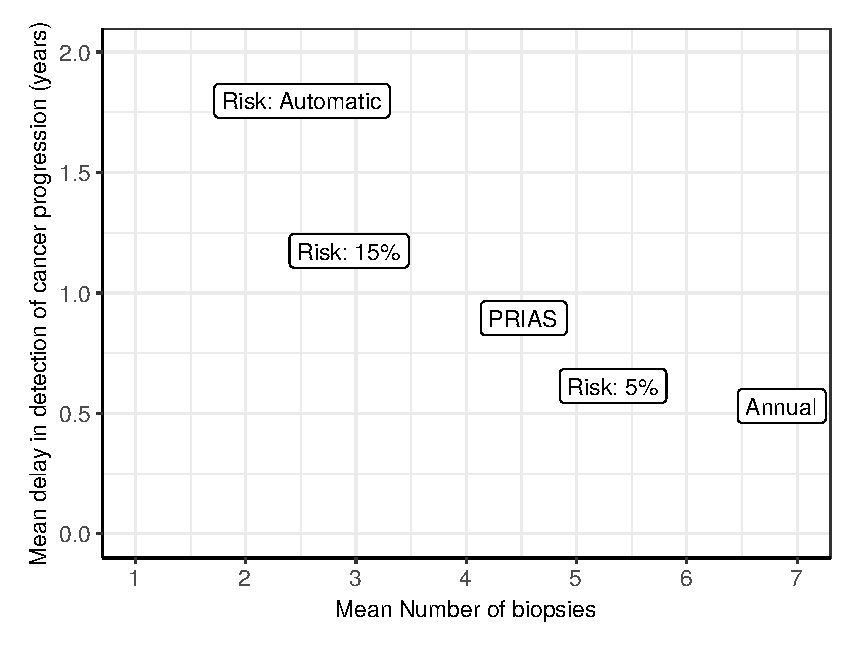
\includegraphics[width=\columnwidth]{images/mean_nb_offset.eps}}
\caption{Mean number of biopsies (of 500 x 250 test patients) scheduled by various biopsy schedules, plotted against the corresponding delay in detection of cancer progression, in years (time of last biopsy - true time of cancer progression). Biopsies are conducted until cancer progression is detected. \textbf{Types of personalized schedules:} Risk:~15\% and Risk:~5\% approaches, schedule biopsy if the risk of cancer progression at a visit is more than 15\% and 5\%, respectively. Risk:~Automatic works similar to Risk:~15\% and Risk:~5\%, except that the risk threshold for biopsy is chosen automatically by maximizing $\mbox{F}_1$ score (see \hyperref[sec:methods]{Methods}). Annual corresponds to a schedule of yearly biopsies and PRIAS corresponds to biopsies as per PRIAS protocol (see \hyperref[sec:introduction]{Introduction}).}
\label{fig:mean_nb_offset}
\end{figure}

Since patients have varying cancer progression speeds, the impact of different approaches for biopsies also varies with the speed. In order to highlight these differences we trichotomize patients into 3 categories (fast, intermediate, slow speed) as per their time of cancer progression. In the simulated patients, we observed that for roughly 50\% of the patients cancer progression did not take place in the 10 year follow-up. These could be seen as patients with a slow speed of cancer progression. Roughly 30\% of the patients obtain cancer progression within first 3.5 years. These could be high risk patients who choose AS instead of immediate treatment, or patients with an initially misdiagnosed state of cancer \cite{cooperberg2011outcomes}. These patients can be considered as fast progressing patients. We consider that the remaining 20\% patients with cancer progression times between 3.5 and 10 years have an intermediate speed of cancer progression. Although such a trichotomization may not be perfect and can only be done retrospectively in a simulation setting, we do it only for the purpose of illustration.

\begin{figure}[!htb]
\captionsetup{justification=justified}
\centerline{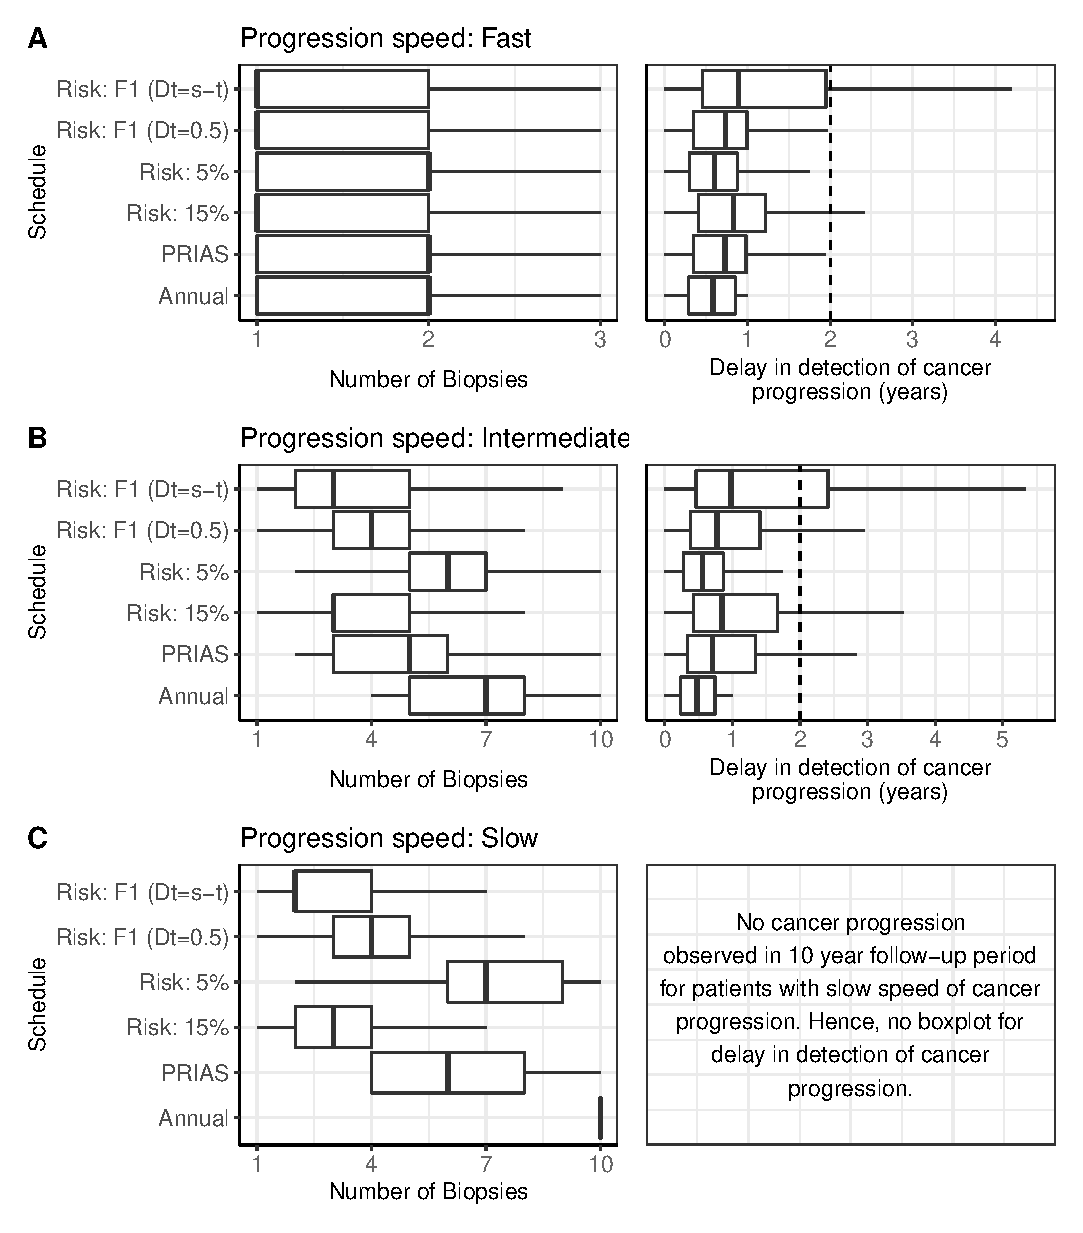
\includegraphics[width=\columnwidth]{images/sim_res_combined.eps}}
\caption{Boxplot showing variation in number of biopsies, and the delay in detection of cancer progression, in years (time of last biopsy - true time of cancer progression) for various biopsy schedules. Biopsies are conducted until cancer progression is detected. \textbf{Panel~A:} results for simulated patients who had a faster speed of cancer progression, with progression times between 0 and 3.5 years. \textbf{Panel~B:} results for simulated patients who had an intermediate speed of cancer progression, with progression times between 3.5 and 10 years. \textbf{Panel~C:} results for simulated patients who did not have cancer progression in the 10 years of follow-up. \textbf{Types of personalized schedules:} Risk:~15\% and Risk:~5\% approaches, schedule biopsy if the risk of cancer progression at a visit is more than 15\% and 5\%, respectively. Risk:~Automatic works similar to Risk:~15\% and Risk:~5\%, except that the risk threshold for biopsy is chosen automatically by maximizing $\mbox{F}_1$ score (see \hyperref[sec:methods]{Methods}). Annual corresponds to a schedule of yearly biopsies and PRIAS corresponds to biopsies as per PRIAS protocol (see \hyperref[sec:introduction]{Introduction}).}
\label{fig:sim_res_combined}
\end{figure}

For faster progressing patients (30\% of the total patients), the boxplots in panel A of Figure~\ref{fig:sim_res_combined} shows the variation in the number of biopsies (of 500 x 250 test patients), and the delay in detection of cancer progression, in years (time of last biopsy - true time of cancer progression) due to various biopsy schedules. We can see that the personalized schedules conduct a median of one biopsy compared to two biopsies for PRIAS and annual schedule. The performance of personalized schedule with 15\% risk threshold is similar to that of PRIAS schedule. Thus with personalized approach, one biopsy may get saved for faster progressing patients.

For patients with intermediate progression speed (20\% of the total patients), the boxplots in panel B of Figure~\ref{fig:sim_res_combined} shows the variation in number of biopsies, and the delay in detection of cancer progression due to various biopsy schedules. Firstly, we can see that personalized schedules with a small risk threshold such as 5\% risk conduct many more biopsies than other personalized schedules. Consequently, their performance with respect to the delay in detection of progression is similar to that of annual schedule. However, personalized schedule with slightly higher risk (15\%) and risk chosen automatically, schedule a median of 3 biopsies each. This is despite the fact that the delay in detection of cancer progression due to the schedule with 15\% risk threshold is similar to that of the PRIAS schedule. However, the PRIAS schedule conducts more biopsies (median of 5 biopsies). Thus, the personalized approach may lead to two less biopsies for patients with intermediate speed of progression.

The patients who are at most advantage with the personalized schedules are the patients who progress slowly (50\% of the total patients). Panel C of Figure~\ref{fig:sim_res_combined} shows a boxplot of the number of biopsies conducted by various biopsy schedules for such patients. It can be seen that the annual schedule may lead to 10 unnecessary biopsies for everyone. The PRIAS schedule, schedules a median of 6 unnecessary biopsies. In comparison the personalized schedules using 15\% risk threshold and automatically chosen risk threshold, schedule only 2 and 3 biopsies, respectively.

% !TEX root =  ../main_manuscript.tex 
\section{Discussion}
We developed a novel methodology for personalized biopsies in low-risk PCa patients enrolled in AS programs. These biopsies are based on a patient's risk profile for having a Gleason $\geq$ 7 (GS7). To assist patients in making a choice between the personalized and currently practiced fixed schedules, we give objective estimates of the consequences of following each schedule. More specifically, for a schedule we give the total number of biopsies (burden), the time at which they will be conducted, and the expected delay in detection of GS7. This delay is estimated after accounting for the probability of not having any GS7 at all over the follow-up period. Lastly, our approach dynamically updates the aforementioned schedules and consequences as more patient data becomes available over follow-up.

The aforementioned methodology is based on the world's largest PCa AS program, PRIAS. Consequently, a lot of patients may get benefited from this study. To this end, we have developed a web-application implementing our methodology. The web-application only requires patient data in well known file formats (e.g., SPSS, CSV etc.), but does not require any separate integration with the electronic health record of the PRIAS program. We hope that this will lead to improvement in the shared decision making of biopsies, with patients having objective estimates of the consequences of their decisions. 

\textbf{Clinical implications:} The median survival time for GS7 is more than ten years in PRIAS. That is, more than 50\% patients do not require any biopsy during the first ten years of follow-up. The situation is similar in many other cohorts. Hence frequent biopsies may not be recommended for all patients.

Existing work on reducing the burden of biopsies in AS primarily advocates less frequent heuristic schedules of biopsies \citep{inoue2018comparative} (e.g., biopsies biennially instead of annually). To our knowledge, risk-based biopsy schedules have barely been explored yet in AS \citep{nieboer2018active,bruinsma2016active}. The part of our results pertaining to the fixed/heuristic schedules is comparable with corresponding results obtained in existing work \citep{inoue2018comparative}, even though the AS cohorts are not the same. Thus, we anticipate similar validity for the results pertaining to the personalized schedules.

Our work has certain limitations. The prediction model that we developed is valid only for the first thirteen years of follow-up in AS, whereas PCa in AS patients progresses slowly. This issue can be mitigated by refitting the model as more follow-up data is gathered in PRIAS. The results of external validation indicate that the use of our model may be restricted in cohorts with AUC, and RMSPE results similar to that of PRIAS. To this end, in other cohorts, refitting the model to their dataset will be required before making risk based schedules, and estimating the consequences of each schedule. There is also a potential for including diagnostic information from novel biomarkers, quality of life measures, and magnetic resonance imaging. Currently, this data is very sparsely available in the PRIAS dataset. However, in future, adding this information in our model is trivial. This is because modeling correlation for extra outcomes  (see Figure \ref{fig:jm_blockdiag}), mainly entails sharing the random effects in the joint model structure. Since MRI scans are expensive in developing countries, our model can also be used to trigger MRI scans. Lastly, in this study focus only on biopsy Gleason upgrade (reclassification). In this regard, accounting for competing risks (see Table \ref{table:prias_summary}), and for inter-observer variation \citep{coley2017prediction} in biopsy Gleason scores can be interesting to investigate further.

% !TEX root =  ../main_manuscript.tex 

\begin{acks}
The first and last Authors would like to acknowledge support by Nederlandse Organisatie voor Wetenschappelijk Onderzoek (the national research council of the Netherlands) VIDI grant nr. 016.146.301, and Erasmus University Medical Center funding. The Authors also thank the Erasmus University Medical Center's Cancer Computational Biology Center for giving access to their IT-infrastructure and software that was used for the computations and data analysis in this study. Lastly, we thank Joost Van Rosmalen from the Department of Biostatistics, Erasmus University Medical Center, for feedback on the manuscript.
\end{acks}

\begin{dci}
The Authors declare that there is no conflict of interest.
\end{dci}

\begin{sm}
Supplementary material for this article are available after references and figures in this document.
\end{sm} 

\bibliographystyle{SageV}
\bibliography{bibliography.bib}

\end{document}


